\chapter{Gestion d'affectations : AffectBundle}

Ce bundle contient toutes les fonctionnalités en rapport à l'affectation des étudiants.
Elles interviennent principalement du côté Admin, car c'est leur rôle d'affecter les élèves. Il y a deux moyens de le faire : l'affectation manuelle et l'algorithme d'affectation automatique.

\section{Affectation manuelle}

L'Admin peut, depuis la page d'accueil, avoir accès à la page d'un étudiant. 
 \bigbreak
 \begin{figure}[H]
	\centering
 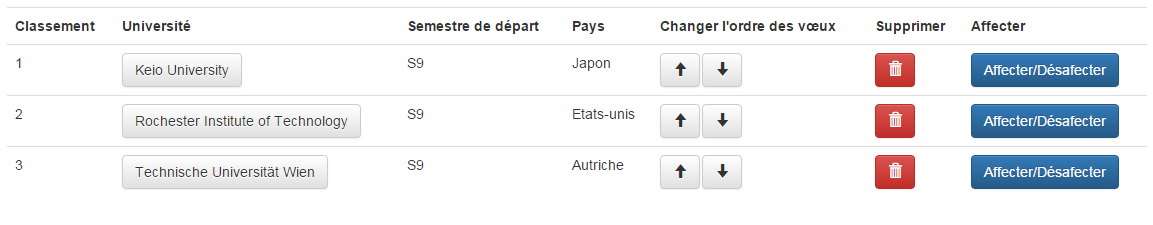
\includegraphics[scale=0.5]{images/voeux_etud_vupar_admin.PNG}
	\caption{Page d'accueil administrateur}
	\label{gm}
\end{figure}
 
\bigbreak
D'ici, il peut affecter ou désaffecter manuellement l'étudiant à un se ses vœux.
Ce choix est alors enregistré et affiché comme la destination de l'étudiant.

Les élèves affectés manuellement ne sont pas pris en compte dans l'algorithme d'affectation.

\section{Algorithme d'affectation suivant le classement}

L'Admin accède à cette fonctionnalité en cliquant sur le lien "Gérer les affectations" depuis sa page d'accueil.
\bigbreak
\begin{figure}[H]
	\centering
	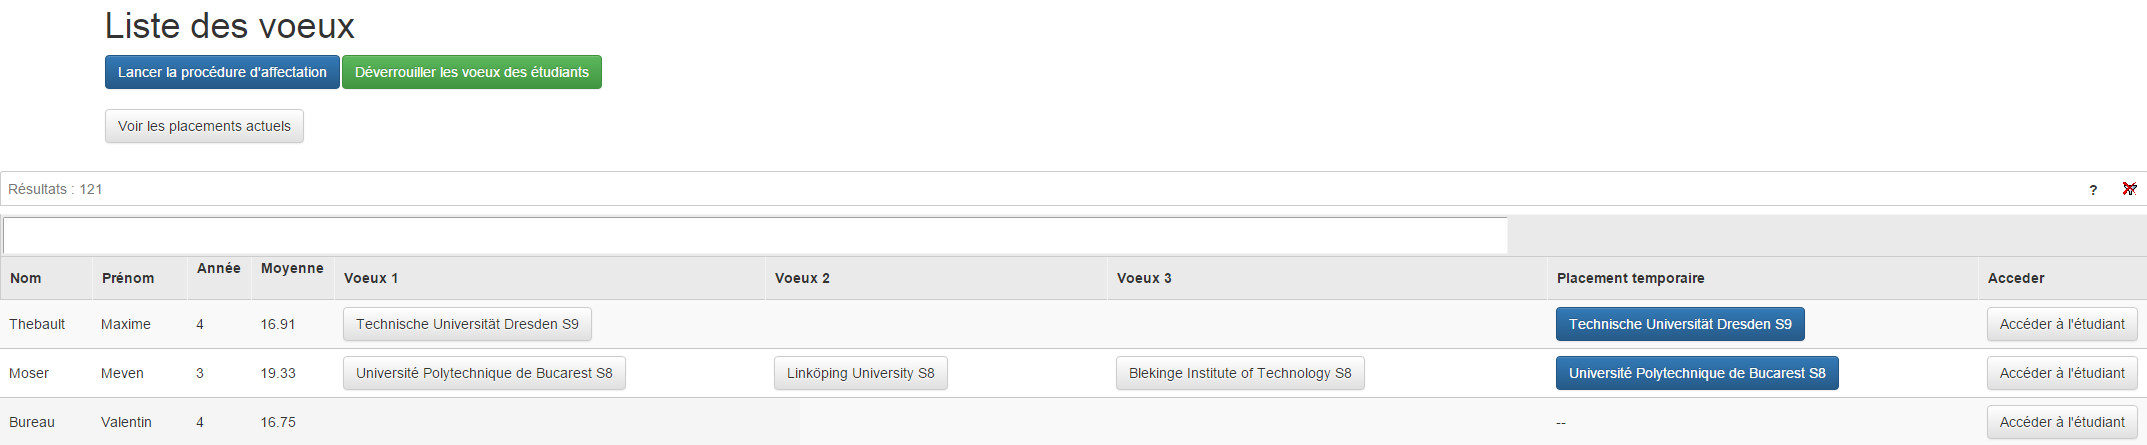
\includegraphics[scale=0.22]{images/Liste_de_voeux_admin.PNG}
	\caption{Page de gestion des affectations}
	\label{ga}
\end{figure}
\bigbreak
L'algorithme prend les élèves à affecter (ceux qui ne sont pas affectés manuellement et qui ont fait des vœux) dans un certain classement. Chaque année est classée selon la moyenne des élèves, puis un classement commun est créé en alternant 4A et 3A (en commençant pas les 4A). Le premier de 4A est suivi du premier de 3A, puis du second de 4A etc.

L'algorithme affecte ensuite les destination en fonction de ce classement.
Une fois fini, le responsable RI peut encore modifier le tableau, puis valide les affectations.

